\documentclass[prb,11pt,tightenlines,twocolumn,aps]{revtex4-1}

\usepackage{amsmath}    % need for subequations
\usepackage{graphicx}   % need for figures
\usepackage{verbatim}   % useful for program listings
\usepackage{color}      % use if color is used in text
\usepackage{subfigure}  % use for side-by-side figures
\usepackage{hyperref}   % use for hypertext links, including those to external
                        % documents and URLs 
\usepackage{blindtext}  % fill text
\usepackage{color}
\usepackage{multirow}
% \usepackage{showframe}
\usepackage[inline]{showlabels}

\raggedbottom           % don't add extra vertical space

\begin{document}

\title{Pure Spin Current Injection in Hydrogenated Graphene Structures}
\author{Reinaldo Zapata-Pe\~na\textsuperscript{1},
        Bernardo S. Mendoza\textsuperscript{1},
        Anatoli I. Shkrebtii\textsuperscript{2}}
\affiliation{\textsuperscript{1}Centro de Investigaciones en \'Optica, Le\'on,
Guanajuato 37150, M\'exico}
\affiliation{\textsuperscript{2}University of Ontario, Institute of Technology,
Oshawa, ON, L1H 7L7, Canada}

\date{\today}

\begin{abstract}
\blindtext
\end{abstract}

\maketitle

%%%%%%%%%%%%%%%%%%%%%%%%%%%%%%%%%%%%%%%%%%%%%%%%%%%%%%%%%%%%%%%%%%%%%%%%%%%%%%
%%%%%%%%%%%%%%%%%%%%%%%%%%%%%%%%%%%%%%%%%%%%%%%%%%%%%%%%%%%%%%%%%%%%%%%%%%%%%%
%%%%%%%%%%%%%%%%%%%%%%%%%%                         %%%%%%%%%%%%%%%%%%%%%%%%%%%
%%%%%%%%%%%%%%%%%%%%%%%%%% I N T R O D U C T I O N %%%%%%%%%%%%%%%%%%%%%%%%%%%
%%%%%%%%%%%%%%%%%%%%%%%%%%                         %%%%%%%%%%%%%%%%%%%%%%%%%%%
%%%%%%%%%%%%%%%%%%%%%%%%%%%%%%%%%%%%%%%%%%%%%%%%%%%%%%%%%%%%%%%%%%%%%%%%%%%%%%
%%%%%%%%%%%%%%%%%%%%%%%%%%%%%%%%%%%%%%%%%%%%%%%%%%%%%%%%%%%%%%%%%%%%%%%%%%%%%%

\section{Introduction}
\blindtext
\begin{figure}[ht!]
    \centering
    \subfigure[\ $xz$ plane view]
    {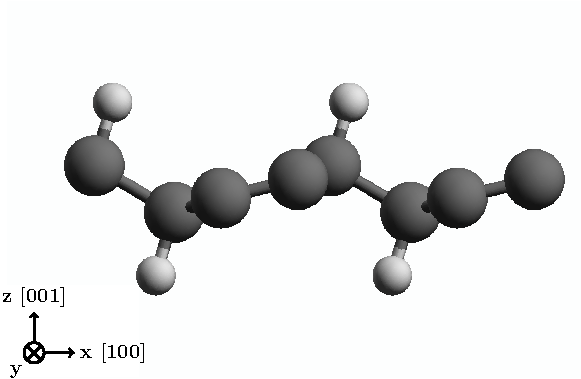
\includegraphics[width=\linewidth]{figures/altstruc2}}
    \label{fig:alt-struc-xz}
    \\
    \subfigure[\ $xy$ plane view]
    {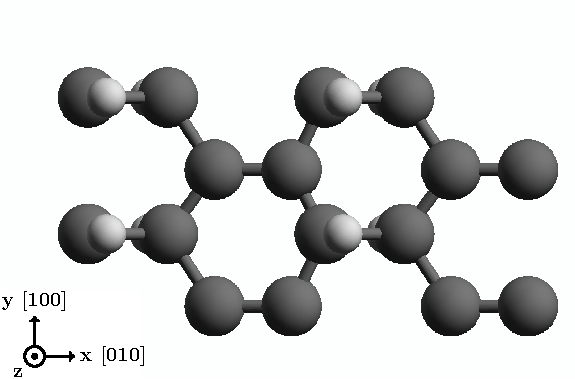
\includegraphics[width=\linewidth]{figures/altstruc1}}
    \label{fig:alt-struc-xy}
    \caption{Alt structure.}
    \label{fig:alt-struc}
\end{figure}
\begin{figure}[ht!]
    \centering
    \subfigure[\ $xz$ plane view]
    {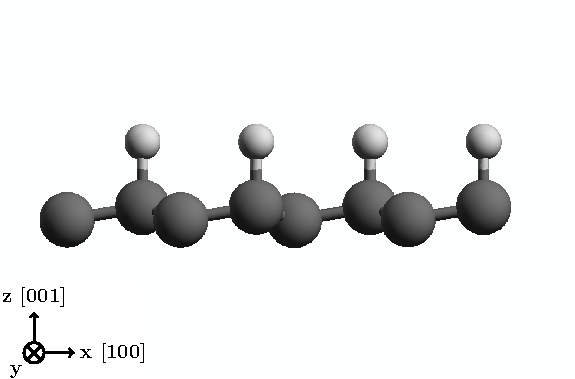
\includegraphics[width=\linewidth]{figures/upstruc2}}
    \label{fig:up-struc-xz}
    \\
    \subfigure[\ $xy$ plane view]
    {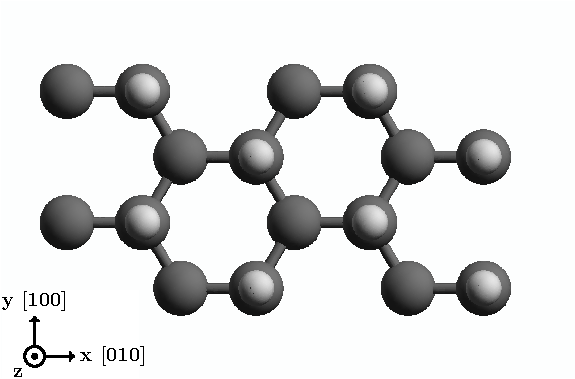
\includegraphics[width=\linewidth]{figures/upstruc1}}
    \label{fig:up-struc-xy}
    \caption{Up structure}
    \label{fig:up-struc}
\end{figure}
\blindtext
\blindtext

\blindtext

%%%%%%%%%%%%%%%%%%%%%%%%%%%%%%%%%%%%%%%%%%%%%%%%%%%%%%%%%%%%%%%%%%%%%%%%%%%%%%
%%%%%%%%%%%%%%%%%%%%%%%%%%%%%%%%%%%%%%%%%%%%%%%%%%%%%%%%%%%%%%%%%%%%%%%%%%%%%%
%%%%%%%%%%%%%%%%%%%%%%%%%%%%%%%%               %%%%%%%%%%%%%%%%%%%%%%%%%%%%%%%
%%%%%%%%%%%%%%%%%%%%%%%%%%%%%%%%  T H E O R Y  %%%%%%%%%%%%%%%%%%%%%%%%%%%%%%%
%%%%%%%%%%%%%%%%%%%%%%%%%%%%%%%%               %%%%%%%%%%%%%%%%%%%%%%%%%%%%%%%
%%%%%%%%%%%%%%%%%%%%%%%%%%%%%%%%%%%%%%%%%%%%%%%%%%%%%%%%%%%%%%%%%%%%%%%%%%%%%%
%%%%%%%%%%%%%%%%%%%%%%%%%%%%%%%%%%%%%%%%%%%%%%%%%%%%%%%%%%%%%%%%%%%%%%%%%%%%%%

\section{Theory} % (fold)
\label{sec:theory}


%%%%%%%%%%%%%%%%%%%%%%%%%%%%%%%%%%%%%%%%%%%%%%%%%%%%%%%%%%%%%%%%%%%%%%%%%%%%%%
%%%%%%%%%%%%%%%%%%%%%%%%%%% Theory: Spin velocity %%%%%%%%%%%%%%%%%%%%%%%%%%%%
%%%%%%%%%%%%%%%%%%%%%%%%%%%%%%%%%%%%%%%%%%%%%%%%%%%%%%%%%%%%%%%%%%%%%%%%%%%%%%


\subsection{Pure spin velocity} % (fold)
\label{sec:theory-pure_spin_current}

The spin density injection current $\dot{K}^{\mathrm{ab}}$ with speed along
direction $\mathrm{a}$ and spin polarization along $\mathrm{b}$ is defined as
\begin{equation}
\dot{K}(\omega) = \mu^{\mathrm{abcd}}(\omega)
E^{\mathrm{c}}(\omega) E^{\mathrm{d*}}(\omega)
\label{eq:dotk}
\end{equation}
where
\begin{widetext}
\begin{align}
\mu^{\mathrm{abcd}} (\omega) 
&=
\frac{\pi e^{2}}{\hbar^{2}} \int 
\frac{d^{3}K}{8 \pi^{3}} \sum_{vcc'}^{'}
\mathrm{Re} \left[ K^{\mathrm{ab}}_{cc'} ( 
r^{\mathrm{c}}_{vc'} 
r^{\mathrm{d}}_{cv } +
r^{\mathrm{d}}_{vc'} 
r^{\mathrm{c}}_{cv } ) \right]
\delta(\omega-\omega_{cv})
\label{eq:mu}
\\
K^{\mathrm{ab}}_{mn}
&=
\sum_{\ell}v^{\mathrm{a}}_{nl} S^{\mathrm{b}}_{lm}
\label{eq:velspi-matelem}
\end{align}
\end{widetext}
is the corresponding spin density injection current pseudotensor. The $'$
in the sum means that $c$ and $c'$ are quasi degenerate states and the sum only
covers these states.

Now we define the spin velocity, $\mathcal{V}^{\mathrm{ab}}$ as the speed at
which the spin polarized in the $\mathrm{b}$   direction moves along the
$\mathrm{a}$ direction when a normal incident beam reaches the $xy$ plane with a
polarization angle $\alpha$. Then,
\begin{widetext}
\begin{align}
\mathcal{V}^{\mathrm{ab}}(\omega,\alpha)
&= \frac{2}{\hbar}
\frac{\mu^{\mathrm{abxx}}(\omega)
E^{2}(\omega)\cos^{2}(\alpha) + 
\mu^{\mathrm{abyy}}(\omega)
E^{2}(\omega)\sin^{2}(\alpha) + 
2\mu^{\mathrm{abxy}}(\omega)
E^{2}(\omega)\cos(\alpha)\sin(\alpha)}
{\xi^{\mathrm{xx}}(\omega)
E^{2}(\omega)\cos^{2}(\alpha) + 
\xi^{\mathrm{yy}}(\omega)
E^{2}(\omega)\sin^{2}(\alpha)},
\nonumber \\
&= \frac{2}{\hbar}
\frac{\mu^{\mathrm{abxx}}(\omega)\cos^{2}(\alpha) + 
\mu^{\mathrm{abyy}}(\omega)\sin^{2}(\alpha) + 
\mu^{\mathrm{abxy}}(\omega)\sin(2\alpha)}
{\xi^{\mathrm{xx}}(\omega)\cos^{2}(\alpha) + 
\xi^{\mathrm{yy}}(\omega)\sin^{2}(\alpha)}.
\label{eq:vab}
\end{align}
\end{widetext}

For an angle $\alpha = \frac{\pi}{4}$ this expression can be reduced to 
\begin{align}
\mathcal{V}^{\mathrm{ab}} (\omega)
&= \frac{2}{\hbar}
\frac{\mu^{\mathrm{abxx}}(\omega) + \mu^{\mathrm{abyy}}(\omega) + 
2\mu^{\mathrm{abxy}}(\omega)}
{\xi^{\mathrm{xx}}(\omega) + \xi^{\mathrm{yy}}(\omega)}.
\label{eq:vab-90deg}
\end{align}


%%%%%%%%%%%%%%%%%%%%%%%%%%%%%%%%%%%%%%%%%%%%%%%%%%%%%%%%%%%%%%%%%%%%%%%%%%%%%%
%%%%%%%%%%%%%%%%%%%%%%%%%%%% Theory: Fixing spin %%%%%%%%%%%%%%%%%%%%%%%%%%%%%
%%%%%%%%%%%%%%%%%%%%%%%%%%%%%%%%%%%%%%%%%%%%%%%%%%%%%%%%%%%%%%%%%%%%%%%%%%%%%%


\subsection{Fixing spin}\label{sec:theory-fixspin}
Considering that we have 2D structures we can fix the spin direction along the
$x$, $y$, and $z$ Cartesian coordinates and then define the magnitude of the
spin velocity $|\mathcal{V}_{\sigma^{\mathrm{b}}}(\omega,\alpha)|$ in a fixed angle $\gamma_{\mathrm{b}}(\omega,\alpha)$ as
\begin{align}
|\mathcal{V}_{\sigma^{\mathrm{b}}}(\omega,\alpha)| 
&=
\sqrt{
[\mathcal{V}^{\mathrm{ax}}(\omega,\alpha)]^{2}\ +
[\mathcal{V}^{\mathrm{ay}}(\omega,\alpha)]^{2}\ 
}, 
\label{eq:vs-mag}
\\
\gamma_{\mathrm{b}} (\omega,\alpha)
&=
\tan^{-1} \left( \frac{\mathcal{V}^{\mathrm{ay}}(\omega,\alpha)}
{\mathcal{V}^{\mathrm{ax}}(\omega,\alpha)} \right),
\label{eq:gamma-ang}
\end{align}
where the angle is measured in the counter-clockwise direction from the positive
$x$ axis.


%%%%%%%%%%%%%%%%%%%%%%%%%%%%%%%%%%%%%%%%%%%%%%%%%%%%%%%%%%%%%%%%%%%%%%%%%%%%%%
%%%%%%%%%%%%%%%%%%%%%%%%%%%% Theory: Fixing vel %%%%%%%%%%%%%%%%%%%%%%%%%%%%%%
%%%%%%%%%%%%%%%%%%%%%%%%%%%%%%%%%%%%%%%%%%%%%%%%%%%%%%%%%%%%%%%%%%%%%%%%%%%%%%


\subsection{Fixing velocity.}\label{sec:theory-fixvel}

In a similar way we can fix the velocity in the $xy$ plane
along $x$ and $y$ directions and define $|\mathcal{V}^{\mathrm{a}}(\omega,\alpha)|$ as
\begin{align}
|\mathcal{V}^{\mathrm{a}}&(\omega,\alpha)| = \nonumber \\
&\sqrt { 
[\mathcal{V}^{\mathrm{ax}}(\omega,\alpha)]^{2} +
[\mathcal{V}^{\mathrm{ay}}(\omega,\alpha)]^{2} +
[\mathcal{V}^{\mathrm{az}}(\omega,\alpha)]^{2} 
},
\label{eq:vv-mag}
\end{align}
and the corresponding polar and azimuthal angles $\theta$ and $\varphi$ as
\begin{align}
\theta_{\mathrm{a}}  (\omega,\alpha)
=& 
\cos^{-1} \left( \frac{\mathcal{V}^{\mathrm{az}}(\omega,\alpha)}
{|\mathcal{V}^{\mathrm{a}}(\omega,\alpha)|} \right),
& 0 \leq &\theta \leq \pi, 
\label{eq:polar-ang}
\\
\varphi_{\mathrm{a}} (\omega,\alpha)
=& 
\tan^{-1} \left( \frac{\mathcal{V}^{\mathrm{ay}}(\omega,\alpha)}
{\mathcal{V}^{\mathrm{ax}}(\omega,\alpha)} \right),
& 0 \leq &\varphi \leq 2\pi.
\label{eq:azimuthal-ang} 
\end{align}


%%%%%%%%%%%%%%%%%%%%%%%%%%%%%%%%%%%%%%%%%%%%%%%%%%%%%%%%%%%%%%%%%%%%%%%%%%%%%%
%%%%%%%%%%%%%%%%%%%%%%%%%% Theory: Layer by layer %%%%%%%%%%%%%%%%%%%%%%%%%%%%
%%%%%%%%%%%%%%%%%%%%%%%%%%%%%%%%%%%%%%%%%%%%%%%%%%%%%%%%%%%%%%%%%%%%%%%%%%%%%%


\subsection{Layer-by-layer analysis.}\label{sec:theory-layer}

For a layered system we have that the total contribution of Eqns. 
\eqref{eq:vs-mag} and \eqref{eq:vv-mag} is given \cite{arzatePRB14} by 

\begin{align}
|\mathcal{V}_{\sigma^{\mathrm{b}}}(\omega,\alpha)|
=& 
\ell_{\mathrm{eff}}
\sum_{\ell=1}^{N_{\mathrm{eff}}}
|\mathcal{V}_{\sigma^{\mathrm{b}}} (\ell | \omega,\alpha)|
\label{eq:vs-layer}
\\
|\mathcal{V}^{\mathrm{a}}(\omega,\alpha)|
=&
\ell_{\mathrm{eff}}
\sum_{\ell=1}^{N_{\mathrm{eff}}}
|\mathcal{V}^{\mathrm{a}} (\ell | \omega,\alpha)|
\label{eq:vv-layer}
\end{align}


%%%%%%%%%%%%%%%%%%%%%%%%%%%%%%%%%%%%%%%%%%%%%%%%%%%%%%%%%%%%%%%%%%%%%%%%%%%%%%
%%%%%%%%%%%%%%%%%%%%%%%%%%%%%%%%%%%%%%%%%%%%%%%%%%%%%%%%%%%%%%%%%%%%%%%%%%%%%%
%%%%%%%%%%%%%%%%%%%%%%%%%%%%%                   %%%%%%%%%%%%%%%%%%%%%%%%%%%%%%
%%%%%%%%%%%%%%%%%%%%%%%%%%%%%   R E S U L T S   %%%%%%%%%%%%%%%%%%%%%%%%%%%%%%
%%%%%%%%%%%%%%%%%%%%%%%%%%%%%                   %%%%%%%%%%%%%%%%%%%%%%%%%%%%%%
%%%%%%%%%%%%%%%%%%%%%%%%%%%%%%%%%%%%%%%%%%%%%%%%%%%%%%%%%%%%%%%%%%%%%%%%%%%%%%
%%%%%%%%%%%%%%%%%%%%%%%%%%%%%%%%%%%%%%%%%%%%%%%%%%%%%%%%%%%%%%%%%%%%%%%%%%%%%%

\section{Results} % (fold)
\label{sec:results}

\begin{table}[t]
\center
\begin{tabular}{ccccc}\\
\hline
\quad Layer \quad & \quad Atom \qquad & \multicolumn{3}{c}{Position [\AA]} \\
\cline{3-5}
\quad No.   \quad & \quad type \qquad & $x$ & $y$ & $z$  \\
\hline
1 & H &  -0.61516 &  -1.42140 & \ 1.47237 \\
2 & C &  -0.61516 &  -1.73300 & \ 0.39631 \\
3 & C & \ 0.61516 & \ 1.73300 & \ 0.15807 \\
4 & C & \ 0.61516 & \ 0.42201 &  -0.15814 \\
5 & C &  -0.61516 &  -0.37396 &  -0.39632 \\
6 & H &  -0.61516 &  -0.68566 &  -1.47237 \\
\hline
\end{tabular}

\caption{Unit cell of \emph{alt} structure. Layer division, atom types and
positions for the \emph{alt} structure. The structure unit cell was divided in
six layers corresponding each one to atoms in different $z$ positions. The
corresponding layer atom position is depicted in Fig. \ref{fig:alt-struc} with
the corresponding number of layer.}
\label{tab:alt-unitcell}
\end{table}
% 
\begin{table}[t]
\center
\begin{tabular}{ccccc}\\
\hline
\quad Layer \quad & \quad Atom \qquad & \multicolumn{3}{c}{Position [\AA]} \\
\cline{3-5}
\quad No.   \quad & \quad type \qquad & $x$ & $y$ & $z$  \\
\hline
1 & H & -0.61516 & -1.77416 &  0.73196 \\
1 & H &  0.61518 &  0.35514 &  0.73175 \\
2 & C & -0.61516 & -1.77264 & -0.49138 \\
2 & C & -0.61516 & -0.35600 & -0.72316 \\
2 & C &  0.61516 &  0.35763 & -0.49087 \\
\hline
\end{tabular}

\caption{Unit cell of \emph{up} structure. Layer division, atom types and
positions for the \emph{up} structure. The structure unit cell was divided in
two layers corresponding to hydrogen and carbon atoms.The corresponding layer
atom position is depicted in Fig. \ref{fig:up-struc} with the corresponding
number of layer.}
\label{tab:up-unitcell}
\end{table}

We preset the results for $|\mathcal{V}^{\mathrm{a}}(\omega,\alpha)|$ and
$|\mathcal{V}_{\sigma^{\mathrm{b}}}(\omega,\alpha)|$ for the C$_{16}$H$_{8}$-alt
and C$_{16}$H$_{8}$-up structures being both noncentrosymmetric semi-infinite 2D
carbon systems with 50\% hydrogenation in different arrangements. The \emph{alt}
system has alternating hydrogen atoms on the upper and bottom sides of the
carbon sheet, while the \emph{up} system has H only on the upper side. We take
the hexagonal carbon lattice to be on the $xy$ plane for both structures, and
the carbon-hydrogen bonds on the perpendicular $xz$ plane, as depicted in Figs.
\ref{fig:alt-struc} and \ref{fig:up-struc}.

We calculated the self-consistent ground state and the Kohn-Sham states using
density functional theory in the local density approximation (DFT-LDA) with a
planewave basis using the ABINIT code \cite{gonzeCPC09}. We used 
Hartwigsen-Goedecker-Hutter (HGH) relativistic separable dual-space Gaussian
pseudopotentials \cite{hartwigsenPRB98} including the spin-orbit interaction
needed to calculate $\mu^{\mathrm{abcd}}(\omega,\alpha)$ presented in Eq.
\eqref{eq:mu}.
% 
It is known that using DFT-LDA to calculate the electronic structure of
materials predict a different band gap than the obtained experimentally. A
correction for the band gap energy value can be calculated by other 
\emph{ab-initio} methods such as the GW approximation \cite{onidaRMP02} but this
is outside the scope of this paper.
% 
The convergence parameters for the calculations of our results corresponding to
the \emph{alt} and \emph{up} structures are cutoff energies of 65\,Ha and
40\,Ha, respectively. The energy eigenvalues and matrix elements were calculated
using 14452 $\mathbf{k}$ points and 8452 $\mathbf{k}$ points in the irreducible
Brillouin zone (IBZ) and present LDA energy band gaps of 0.72\,eV and 0.088\,eV,
respectively for the \emph{alt} and \emph{up} structures. 


%%%%%%%%%%%%%%%%%%%%%%%%%%%%%%%%%%%%%%%%%%%%%%%%%%%%%%%%%%%%%%%%%%%%%%%%%%%%%%
%%%%%%%%%%%%%%%%%%%%%%%%%%% Results: Spin velocity %%%%%%%%%%%%%%%%%%%%%%%%%%%
%%%%%%%%%%%%%%%%%%%%%%%%%%%%%%%%%%%%%%%%%%%%%%%%%%%%%%%%%%%%%%%%%%%%%%%%%%%%%%

\subsection{Spin velocity} % (fold)
\label{sec:res-spin_velocity}

\begin{table}[b]
\begin{tabular}{cccccc}
\hline
\multirow{2}{*}{Structure \quad} & 
Kind of \quad & 
Pol. &
Energy & 
\multicolumn{2}{c}{$\mathcal{V}^{\mathrm{ab}}(\omega,\alpha)$}\\
\cline{5-6}
& system & Ang. & [eV] & $\mathrm{ab}$ \quad & [Km/s]\\
\hline
\emph{up}    & 2D   & 40    & 0.09  & $\mathrm{yz}$ &  87.16    \\
             &      &       & 1.94  & $\mathrm{yz}$ &  22.22    \\
             &      &       & 1.97  & $\mathrm{yz}$ & -29.70    \\
\emph{alt}   & 2D   & 145   & 0.72  & $\mathrm{yz}$ & -40.21    \\
             &      &       & 0.91  & $\mathrm{yz}$ & -32.89    \\
 CdSe        & bulk & 90    & 0.91  & $\mathrm{zz}$ & -26.87    \\
 GaAs        & bulk & 90    & 2.31  & $\mathrm{xx}$ & -21.62    \\
\hline
\end{tabular}

\caption{Comparison of the reported maxima values of
$\mathcal{V}^{\mathrm{ab}}$ for different structures and the corresponding
polarization angle $\alpha$ and energy values.}
\label{tab:vab-str-comp}
\end{table}

%%%%%%%%%%%%%%%%%%%%%%%%%%%%%%%%%%%%%%%%%%%%%%%%%%%%%%%%%%%%%%%%%%%%%%%%%%%%%%
%%%%%%%%%%%%%%%%%%%%%%%%%% Res: mu & V^{ab} comparison %%%%%%%%%%%%%%%%%%%%%%%
\begin{figure}[t]
    \centering
    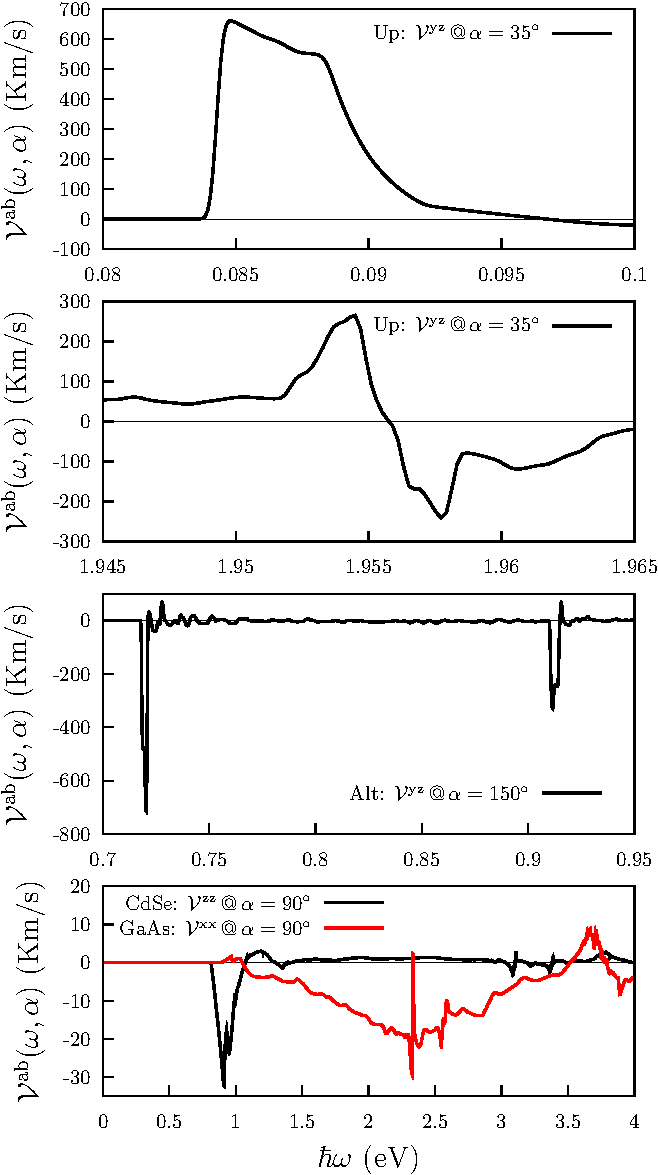
\includegraphics[width=\linewidth]{plots/vab-str-comp}
    
    \caption{Comparison of most intense responses of $\mathcal{V}^{\mathrm{ab}}$
    for 2D \emph{alt} and \emph{up}, and bulk CdSe and GaAs structures and the
    corresponding polarization angles.}
    \label{fig:vab-str-comp}
\end{figure}

{\Large  We calculated the $\mathcal{V}^{\mathrm{ab}}(\omega,\alpha)$} response In figure
\ref{fig:vab-str-comp} we present a comparison of the most intense responses
resulting from evaluate the Eq. \eqref{eq:vab} for the \emph{alt} and \emph{up}
2D structures and CdSe and GaAs bulk systems. As we can see from this figure the
most intense response corresponds to the \emph{up} structure centered at
0.088\,eV corresponding to the Far Infrared (FIR) radiation and reaching a spin
velocity of 87.2\,Km/s.
% 
In the other hand, for an energy range from 0.66\,eV to 3.0\,eV, corresponding
to energies of the Near Infrared (NIR) and visible radiation, all the four
structures have contributions in the same order of magnitude.
% 
Starting with the 2D structures we have that the \emph{up} structure has other
two peaks centered at 1.94\,eV and 1.97\,eV reaching spin velocities of
22.2\,Km/s and -29.7\,Km/s, respectively, and the \emph{alt} structure has two
peaks centered at 0.72\,eV and 0.91\,eV reaching spin velocities of -40.2\,Km/s
and -32.9\,Km/s, respectively.
% 
Then, for the bulk structures we have that the CdSe has only one intense
response centered at 0.91\,eV reaching a spin velocity of -26.9\,Km/s, and the
GaAs structure has a large and almost planar zone where the response is held
reaching the maximum for an incoming beam of energy of 2.31\,eV and resulting in
a spin velocity of -21.6\,Km/s.
% 
In table \ref{tab:vab-str-comp} we present the comparison of this values for the
2D and bulk structures. We found that the most intense response for the spin
velocity of the \emph{up} structure is 3.25 times more intense than CdSe and
4.03 times more intense than the GaAs bulk structures. Also, the \emph{alt}
structure has a response more intense than the bulk systems but being less
intense than the corresponding to the \emph{up} one.
% 


%%%%%%%%%%%%%%%%%%%%%%%%%%%%%%%%%%%%%%%%%%%%%%%%%%%%%%%%%%%%%%%%%%%%%%%%%%%%%%
%%%%%%%%%%%%%%%%%%%%%%%%%%%% Results: Fixing spin %%%%%%%%%%%%%%%%%%%%%%%%%%%%
%%%%%%%%%%%%%%%%%%%%%%%%%%%%%%%%%%%%%%%%%%%%%%%%%%%%%%%%%%%%%%%%%%%%%%%%%%%%%%


\subsection{Fixing spin} % (fold)
\label{sec:res-fixspin}


%%%%%%%%%%%%%%%%%%%%%%%%%%%%%%%%%%%%%%%%%%%%%%%%%%%%%%%%%%%%%%%%%%%%%%%%%%%%%%
%%%%%%%%%%%%%%%%%%%%%%%%%%% Res: fixing spin Up  %%%%%%%%%%%%%%%%%%%%%%%%%%%%%

\begin{figure}[t]
    \centering
    \subfigure[\ \label{fig:up-3d-vsz-1}]
    {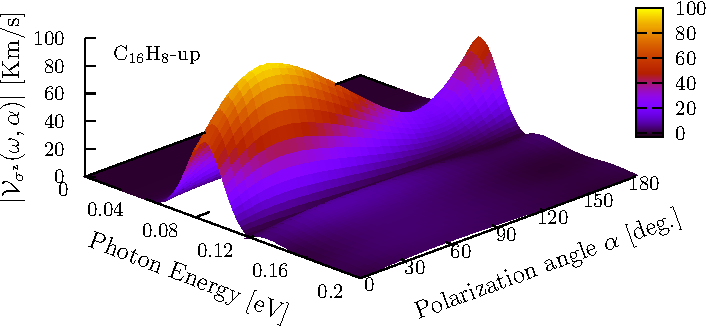
\includegraphics[width=\linewidth]{upplots/up-3d-svaz-1}}
    \\
    \subfigure[\ \label{fig:up-3d-vsz-2}]
    {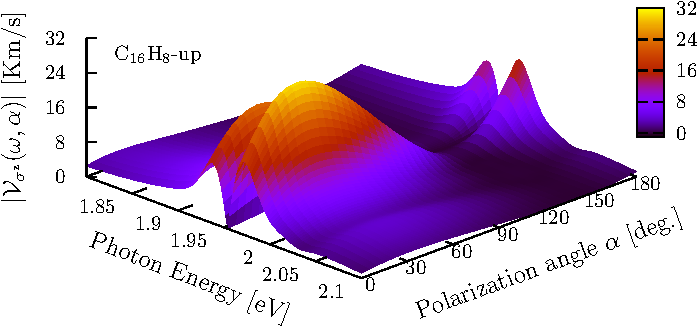
\includegraphics[width=\linewidth]{upplots/up-3d-svaz-2}}

    \caption{$|\mathcal{V}_{\sigma^{\mathrm{z}}}(\omega,\alpha)|$, response
    as a function of the photon energy and polarization angle $\alpha$ for the
    \emph{up} structure for two energy ranges. The absolute maxima is located
    for an energy range from 0.08\,eV to 0.10\,eV and the local maximum from
    1.95\,eV to 2.0\,eV and both for polarization angles between $25^{\circ}$
    and $50^{\circ}$.}
    \label{fig:up-3d-vsz}   
\end{figure}

\begin{figure}[t]
    \centering
    \subfigure[\, \label{fig:up-vaz-rag-1}]
    {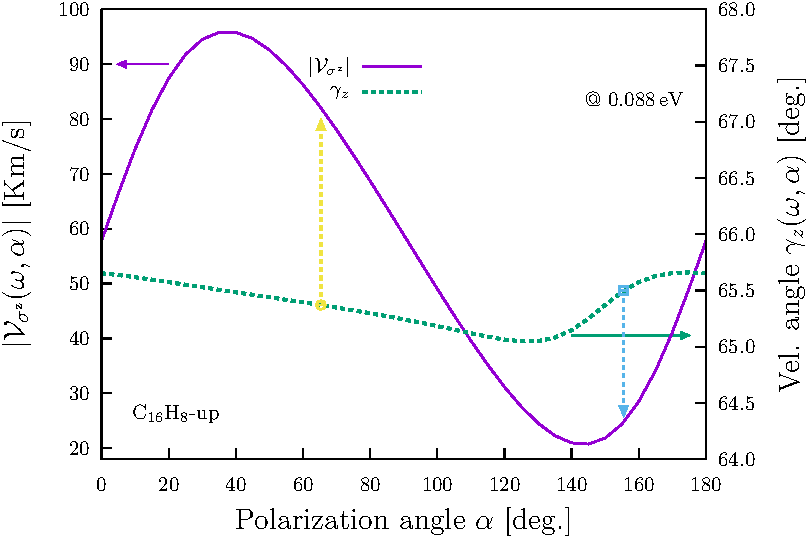
\includegraphics[width=\linewidth]{upplots/up-vaz-rag-1}}
    \\
    \subfigure[\, \label{fig:up-vaz-rag-2}]
    {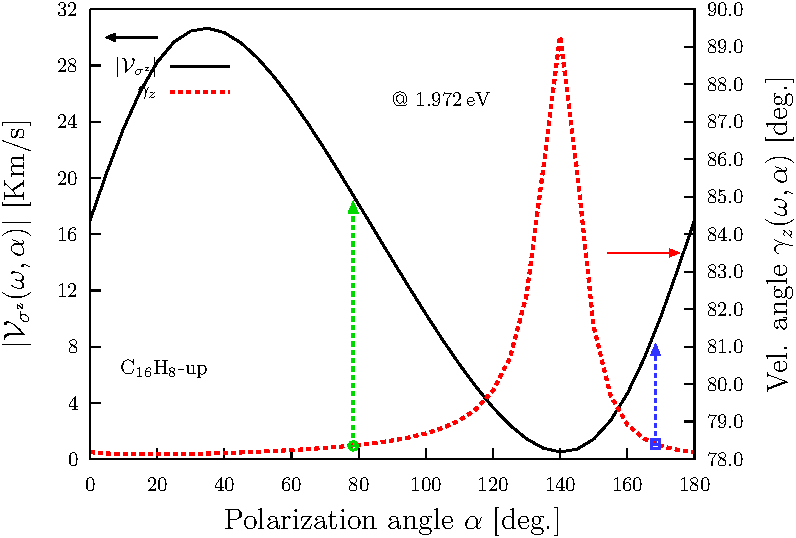
\includegraphics[width=\linewidth]{upplots/up-vaz-rag-2}}

    \caption{Most intense response of
    $|\mathcal{V}_{\sigma^{\mathrm{z}}}(\omega,\alpha)|$ (top frames, right
    scale of figs (a) and (b)), the corresponding velocity angle
    $\gamma_{\mathrm{z}}(\omega,\alpha)$ (top frames, right scale), the
    collinear (circled box) and perpendicular (square box) angles, and the two
    components $\mathcal{V}^{\mathrm{xz}}(\omega,\alpha)$ and
    $\mathcal{V}^{\mathrm{yz}}(\omega,\alpha)$ (bottom frames) for the \emph{up}
    structure fixing the energy to 0.088\,eV. }
    \label{fig:up-vaz-rag}
\end{figure}

% %%%%%%%%%%%%%%%%%
% %% 0.0 eV - 0.16 eV  &  1.80 ev - 2.1 ev
% %% Description of UP |V_{s^z}| 3D
% %%%%%%%%%%%%%%%%%

Using the Eq. \eqref{eq:vs-mag}, we calculated the
$|\mathcal{V}_{\sigma^{\mathrm{b}}}|(\omega,\alpha)$ response and made the
analysis for the case when the spin is fixed in the $z$ direction, directed
perpendicularly to the surface of the \emph{alt} and \emph{up} structures. Also,
using the Eq. \eqref{eq:gamma-ang}, we determined the angle
$\gamma_{\mathrm{b}}(\omega,\alpha)$ where the spin-velocity is directed on the
surface of the each structure.

\textbf{Up structure}

We first analyzed two energy ranges for the \emph{up} structure, the first for
an incoming energy beam from 0.0\,eV to 0.2\,eV which inlude the THz and the Mid
Infrared (MIR) range, where the absolute maximum of the
$|\mathcal{V}_{\sigma^{\mathrm{z}}}(\omega,\alpha)|$ response is obtained and
the second for an energy range from 1.80\,eV to 2.1\,eV, corresponding to
visible radiation, where two local maxima are found.
% 
In Fig. \ref{fig:up-3d-vsz} we present the
$|\mathcal{V}_{\sigma^{\mathrm{z}}}(\omega,\alpha)|$ spectra resulting from
evaluate Eq. \eqref{eq:vs-mag} using different polarization angles $\alpha$ in
Eq. \eqref{eq:vab}. From the figure we have that the onset of the response
starts when the energy of the incoming beam is the same of the gap energy.
% 
Making the analysis, we obtained that the zone where the maximum response is
held corresponds to a energy range of the incident beam from 0.084\,eV to
0.093\,eV and polarization angles $\alpha$ between $30^{\circ}$ and
$45^{\circ}$. Also two local maxima are held for same polarization angles but
for an energy range of the incoming beam between 1.90\,eV and 2.05\,eV.
% %%%%%%%%%%%%%%%%%
% %% 0.0 eV - 0.16 eV
% %% Description of UP |V_{s^z}| & gamma  vs. alpha agle
% %%%%%%%%%%%%%%%%%
In the top frames of Figs.\ref{fig:up-vaz-rag-1} and \ref{fig:up-vaz-rag-2} we
present in solid lines the result of evaluate
$|\mathcal{V}_{\sigma^{\mathrm{z}}}(\omega,\alpha)|$, related to the left scale,
fixing the energy of the incoming beam to 0.088\,eV and 0.912\,eV, respectively,
for which value the response is maximized for the \emph{up} structure. In the
same figures and frames we present in dashed lines, related to the right scale,
the corresponding velocity angle $\gamma_{\mathrm{z}}(\omega,\alpha)$ obtained
from the evaluation of Eq. \eqref{eq:gamma-ang}, and in the bottom frames of
those figures the corresponding components
$\mathcal{V}^{\mathrm{xz}}(\omega,\alpha)$ and
$\mathcal{V}^{\mathrm{yz}}(\omega,\alpha)$. Also we present two circled and
square boxes indicating the values where the angles of the spin velocity are
parallel and perpendicular and the arrows are directed to the value of the
response corresponding to those angles.
% 
From Figs. \ref{fig:up-3d-vsz-1} and \ref{fig:up-vaz-rag-1} we have that the
absolute maximum response for the \emph{up} structure is obtained for an
incoming beam with energy of 0.088\,eV and polarization angle
$\alpha=40^{\circ}$ resulting in a value of
$|\mathcal{V}_{\sigma^{\mathrm{z}}}(\omega,\alpha)|=95.8$\,Km/s coming from the
contribution of the components
$\mathcal{V}^{\mathrm{xz}}(\omega,\alpha)=39.8$\,Km/s and
$\mathcal{V}^{\mathrm{yz}}(\omega,\alpha)=87.2$\,Km/s for the spin polarized in
the $\mathrm{z}$ direction and having a velocity angle
$\gamma_{\mathrm{z}}(\omega,\alpha)=65^{\circ}$ on the $xy$ plane.
% 
In the same figure the green circled box indicates the value for which the
polarization angle $\alpha$ and the response direction angle
$\gamma_{\mathrm{z}}(\omega,\alpha)$ are collinear being both angle
$65.5^{\circ}$ and resulting in a value of the response of
$|\mathcal{V}_{\sigma^{\mathrm{z}}}(\omega,\alpha)|=82.3$\,Km/s indicated by the
upward green arrow.
% 
Also the blue square box indicates the value for which the polarization angle
and the response angle are perpendicular being $\alpha=155.5^{\circ}$ and
$\gamma_{\mathrm{x}}(\omega,\alpha)=65.5^{\circ}$; for this angles the response
has a value of $|\mathcal{V}_{\sigma^{\mathrm{z}}}(\omega,\alpha)|=24.8$\,Km/s
indicated by the blue downward arrow.
% 
The green and blue error bars are fixed for a value of $\pm0.5^{\circ}$ and
then, for variations of this magnitude in $\gamma_{\mathrm{z}}(\omega,\alpha)$
the complete range of $\alpha$ angle is included because this last is almost
constant.
% 
Now from Figs. \ref{fig:up-3d-vsz-2} and \ref{fig:up-vaz-rag-2} we have that a
local maxima of the response is obtained for an incoming beam with energy of
0.912\,eV and same polarization angle $\alpha=40^{\circ}$ resulting in a value
of $|\mathcal{V}_{\sigma^{\mathrm{z}}}(\omega,\alpha)|=30.3$\,Km/s. This comes
from a major contribution of the $\mathcal{V}^{\mathrm{yz}}(\omega,\alpha)$
component being directed in a velocity angle
$\gamma_{\mathrm{z}}(\omega,\alpha)=78^{\circ}$ on the first Cartesian Quadrant
of the $xy$ plane, for the spin polarized in the $z$ direction.
% 
Again the green circled box indicates the value for which the polarization angle
$\alpha$ and the response direction angle $\gamma_{\mathrm{z}}(\omega,\alpha)$
are collinear being both $78.5^{\circ}$ and having a response value of
$|\mathcal{V}_{\sigma^{\mathrm{z}}}(\omega,\alpha)|=23.5$\,Km/s indicated with
the green upward arrow. We found that for variations in the response angle of
$\pm 2^{\circ}$, indicated with the error bars, corresponds a range in the
polarization angle of $0^{\circ} \leq \alpha \leq 122^{\circ}$ having then a
large range for which the direction of the response is directed to this angle.
% 
The blue square box indicates the value for which the polarization angle and the
response angle are perpendicular being $\alpha=168.5^{\circ}$
$\gamma_{\mathrm{z}}(\omega,\alpha)=78.5^{\circ}$ and having a response
$|\mathcal{V}_{\sigma^{\mathrm{z}}}(\omega,\alpha)|=9.0$\,Km/s indicated with
the blue upward arrow. Again, for variations in the response angle of
$\pm2^{\circ}$, indicated with the error bars, corresponds a range in the
polarization angle of $155^{\circ} \leq \alpha \leq 180^{\circ}$ having again a
large range for which the direction of the response is held.
% 
The most interesting case in which the spin is perpendicular to the surface of
the structure and also for the \emph{up} structure the most intense was the
presented before for which the spin is polarized in the $\mathrm{z}$ direction.
We also made the analysis for the cases when the spin polarization is directed
in the $\mathrm{x}$ and $\mathrm{y}$ direction but we do not present the
corresponding plots. For those cases we have that the absolute maxima response
is obtained for an energy of the incoming beam equal to 0.088\,eV and
polarization angle $\alpha=40^{\circ}$ resulting in values of
$|\mathcal{V}_{\sigma^{\mathrm{x}}}(\omega,\alpha)|=37.4$\,Km/s and
$|\mathcal{V}_{\sigma^{\mathrm{y}}}(\omega,\alpha)|=24.8$\,Km/s.

%%%%%%%%%%%%%%%%%%%%%%%%%%%%%%%%%%%%%%%%%%%%%%%%%%%%%%%%%%%%%%%%%%%%%%%%%%%%%%
%%%%%%%%%%%%%%%%%%%%%%%%%%% Res: fixing spin Alt  %%%%%%%%%%%%%%%%%%%%%%%%%%%%

\begin{figure}[tb]
    \centering
    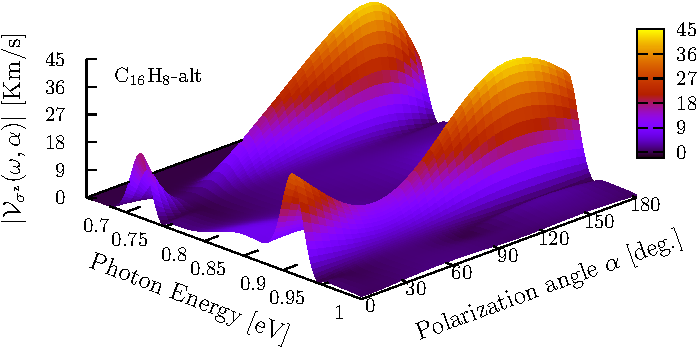
\includegraphics[width=\linewidth]{altplots/alt-3d-svaz}
    \caption{$|\mathcal{V}_{\sigma^{\mathrm{z}}}(\omega,\alpha)|$, response
    vs. photon energy vs. polarization angle $\alpha$ for the \emph{alt}
    structure. The absolute maximum is located for an energy range from 0.90\,eV
    to 0.93\,eV and for polarization angles between $120^{\circ}$ and
    $150^{\circ}$.}
    \label{fig:alt-3d-vsb}
\end{figure}

\begin{figure}[t]
    \centering
    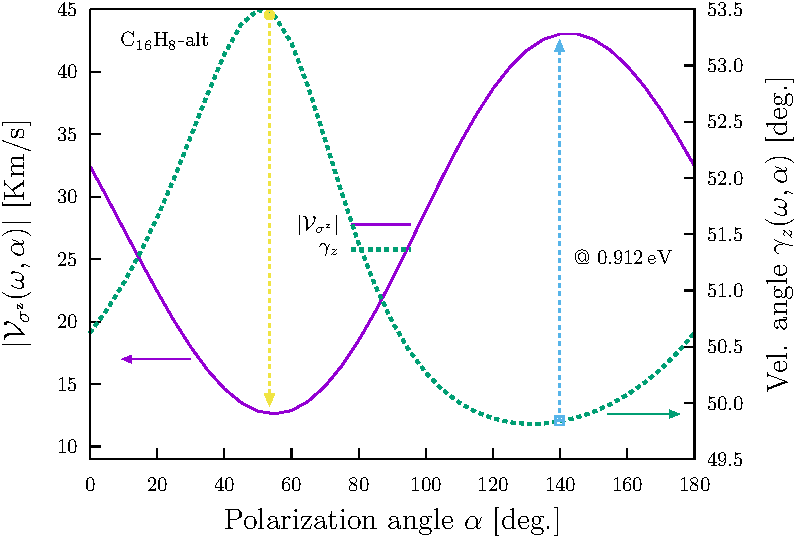
\includegraphics[width=\linewidth]{altplots/alt-vaz-rag}
    \caption{Most intense response of
    $|\mathcal{V}_{\sigma^{\mathrm{z}}}(\omega,\alpha)|$ (top frame, left scale)
    the corresponding velocity angle $\gamma_{\mathrm{z}}(\omega)$ (top frame,
    right scale), the collinear (circled box) and perpendicular (square box)
    angles, and the two components $\mathcal{V}^{\mathrm{xz}}(\omega)$ and
    $\mathcal{V}^{\mathrm{yz}}(\omega)$ (bottom frame) for the \emph{alt}
    structure fixing the energy to 0.912\,eV.}
    \label{fig:alt-vaz-rag}
\end{figure}

% %%%%%%%%%%%%%%%%%
% %% 0.0 eV - 0.16 eV  &  1.80 ev - 2.1 ev
% %% Description of ALT |V_{s^z}| 3D
% %%%%%%%%%%%%%%%%%

\textbf{Alt structure}

For the \emph{alt} structure we analyzed the energy range for the incident beam
from 0.6\,eV to 1.0\,eV, corresponding to the NIR radiation, where the absolute
maximum of $|\mathcal{V}_{\sigma^{\mathrm{z}}}(\omega,\alpha)|$ response is
obtained.
% 
In Fig. \ref{fig:alt-3d-vsb} we present the
$|\mathcal{V}_{\sigma^{\mathrm{z}}}(\omega,\alpha)|$ spectra resulting from
evaluate again Eq. \eqref{eq:vs-mag} and Eq. \eqref{eq:vab} as a function of the
polarization angle $\alpha$ for the \emph{alt} structure.
% 
From this figure we found that the zone where the absolute maximum response is
held corresponds to a energy range from 0.90\,eV to 0.93\,eV and polarization
angles $\alpha$ between $120^{\circ}$ and $150^{\circ}$. Also, a local maximum
is obtained for the same polarization angles but for energies between 0.67\,eV
and 0.75\,eV.
% %%%%%%%%%%%%%%%%%
% %% 0.0 eV - 0.16 eV
% %% Description of ALT |V_{s^z}| & gamma  vs. alpha agle
% %%%%%%%%%%%%%%%%%
In the top frame of Fig. \ref{fig:alt-vaz-rag} we present in solid line the
result of evaluate $|\mathcal{V}_{\sigma^{\mathrm{z}}}(\omega,\alpha)|$, related
to the left scale, fixing the energy of the incoming beam to 0.912\,eV for which
value the response is maximized for the \emph{alt} structure. In the same figure
and frame we present with dashed line, related to the right scale, the velocity
angle $\gamma_{\mathrm{z}}(\omega,\alpha)$ and in the bottom frame the
corresponding $\mathcal{V}^{\mathrm{xz}}(\omega,\alpha)$ and
$\mathcal{V}^{\mathrm{yz}}(\omega,\alpha)$ components. Again, the circled and
square boxes indicate the values for which the polarization angle and the
velocity angle are parallel and perpendicular and with arrows are indicated the
corresponding response value.
% 
From this figure and from Fig. \ref{fig:alt-3d-vsb} we have that the absolute
maximum response for the \emph{alt} structure is obtained for an incoming beam
with polarization angle $\alpha=145^{\circ}$ reaching a velocity of
$|\mathcal{V}_{\sigma^{\mathrm{z}}}(\omega,\alpha)|=43.0$\,Km/s and for the spin
polarized in the $\mathrm{z}$ direction and resulting in a velocity angle
$\gamma_{\mathrm{z}}(\omega,\alpha)=50^{\circ}$ on the first Cartesian Quadrant
of the $xy$ plane. The circled box for the collinear angle corresponds for
angles $\alpha$ and $\gamma_{\mathrm{z}}(\omega,\alpha)$ equal to $53.5^{\circ}$
with a value of $|\mathcal{V}_{\sigma^{\mathrm{z}}}(\omega,\alpha)|=12.7$\,Km/s,
and the blue square box indicates the perpendicular angles for values
$\alpha=140^{\circ}$ and $\gamma_{\mathrm{z}}(\omega,\alpha)=50^{\circ}$ with a
value of $|\mathcal{V}_{\sigma^{\mathrm{z}}}(\omega,\alpha)|=43$\,Km/s. Finally
we found that for variations of $\pm0.5^{\circ}$ of those collinear and
perpendicular angles, presented with the error bars on the boxes, correspond
ranges for the polarization angle $30^{\circ} \leq \alpha \leq 70^{\circ}$ and
$95^{\circ} \leq \alpha \leq 175^{\circ}$ covering a wide range of angles
because the response angle $\gamma_{\mathrm{z}}(\omega,\alpha)$ has small
variations for the complete range of the polarization angle $\alpha$.
% 
Again, for the cases in which the spin polarization is parallel to the surface
of the \emph{alt} structure was calculated but the plots are not presented here.
The absolute maxima for the case when the spin polarization is directed in the
$\mathrm{x}$ and $\mathrm{y}$ direction are obtained for an energy of the
incoming beam equal to 0.912\,eV and polarization angle $\alpha=145^{\circ}$
resulting in values of
$|\mathcal{V}_{\sigma^{\mathrm{x}}}(\omega,\alpha)|=27.1$\,Km/s and
$|\mathcal{V}_{\sigma^{\mathrm{y}}}(\omega,\alpha)|=33.2$\,Km/s.

%%%%%%%%%%%%%%%%%%%%%%%%%%%%%%%%%%%%%%%%%%%%%%%%%%%%%%%%%%%%%%%%%%%%%%%%%%%%%%
%%%%%%%%%%%%%%%%%%%%%%%%%% Results: Fixing velocity %%%%%%%%%%%%%%%%%%%%%%%%%%
%%%%%%%%%%%%%%%%%%%%%%%%%%%%%%%%%%%%%%%%%%%%%%%%%%%%%%%%%%%%%%%%%%%%%%%%%%%%%%


\subsection{Fixing velocity} % (fold)
\label{sec:res-fixvel}


%%%%%%%%%%%%%%%%%%%%%%%%%%%%%%%%%%%%%%%%%%%%%%%%%%%%%%%%%%%%%%%%%%%%%%%%%%%%%%
%%%%%%%%%%%%%%%%%%%%%%%%%%% Res: fixin vel Up  %%%%%%%%%%%%%%%%%%%%%%%%%%%%%%%

Now, using the Eq. \eqref{eq:vv-mag}, we calculated the
$|\mathcal{V}^{\mathrm{a}}(\omega,\alpha)|$ response and made the analysis for
the case when the velocity is fixed in the $x$ and $y$ direction over the
surface of the \emph{alt} and \emph{up} structures. Also, using the Eqns.
\eqref{eq:polar-ang} and \eqref{eq:azimuthal-ang}, we determined the polar
$\theta_{\mathrm{a}}(\omega,\alpha)$ and azimuthal
$\varphi_{\mathrm{a}}(\omega,\alpha)$ angles where the spin polarization is
directed.


\textbf{Up structure.}
\begin{figure}[t]
    \centering
    \subfigure[\ $|\mathcal{V}^{\mathrm{x}}(\omega,\alpha)|$ for \emph{up}
    structure
    \label{fig:up-3d-vvx-1}]
    {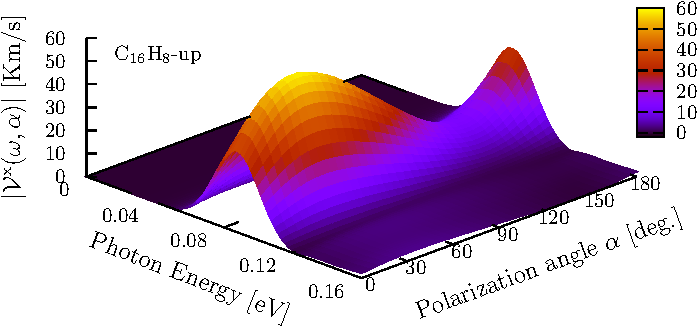
\includegraphics[width=\linewidth]{upplots/up-3d-vxb-1}}
    \\
    \subfigure[\ $|\mathcal{V}^{\mathrm{y}}(\omega,\alpha)|$ for \emph{up}
    structure
    \label{fig:up-3d-vvy-1}]
    {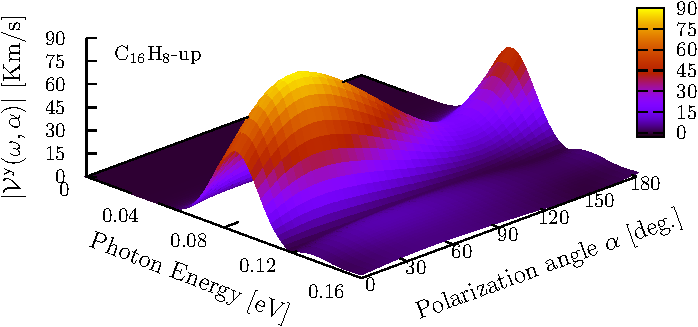
\includegraphics[width=\linewidth]{upplots/up-3d-vyb-1}}
    
    \caption{$|\mathcal{V}^{\mathrm{a}}(\omega,\alpha)|$ response vs. photon
    energy vs. polarization angle for the \emph{up} structure. The absolute
    maxima of both responses $|\mathcal{V}^{\mathrm{x}}(\omega,\alpha)|$ and
    $|\mathcal{V}^{\mathrm{y}}(\omega,\alpha)|$ are localized in the energy
    range from 0.08\,eV to 0.10\,eV and for polarization angles from
    $25^{\circ}$ to $50^{\circ}$.}
    \label{fig:up-3d-vva-1}
\end{figure}
\begin{figure}[t]
    \centering
    \subfigure[\ $|\mathcal{V}^{\mathrm{x}}(\omega,\alpha)|$ 
    \label{fig:up-vx-comp-rtp-1}]
    {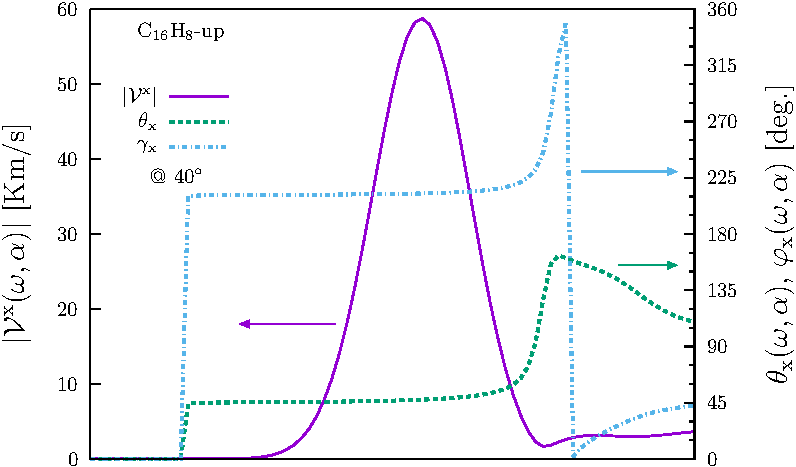
\includegraphics[width=\linewidth]{upplots/up-vxb-rtp-m1}}
    \\
    \subfigure[\ $|\mathcal{V}^{\mathrm{y}}(\omega,\alpha)|$ 
    \label{fig:up-vy-comp-rtp-1}]
    {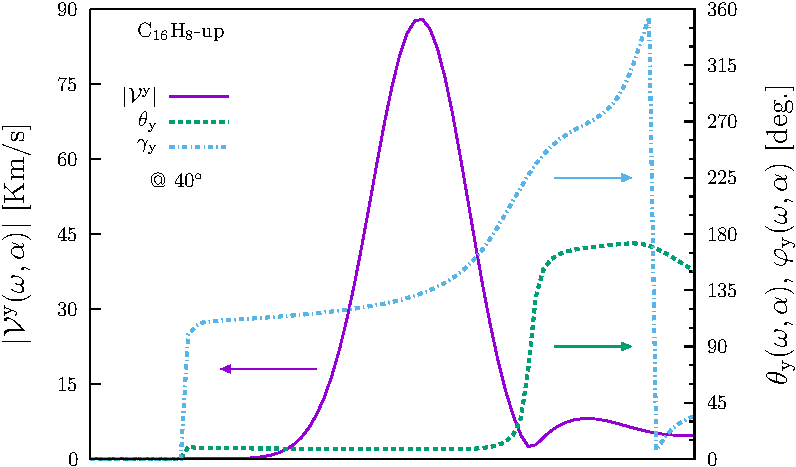
\includegraphics[width=\linewidth]{upplots/up-vyb-rtp-m1}}
    
    \caption{Most intense response of
    $|\mathcal{V}^{\mathrm{x}}(\omega,\alpha)|$ and
    $|\mathcal{V}^{\mathrm{y}}(\omega,\alpha)|$ (top frames left scale of Figs.
    (a) and (b)), the corresponding polar $\varphi$ and azimuthal $\theta$
    angles (top frames right scale), and the corresponding three components
    (bottom frames) for the \emph{up} structure fixing the polarization angle to
    $\alpha=40^{\circ}$ to maximize the response.}
    \label{fig:up-vab-comp-rtp-1}
\end{figure}

% %%%%%%%%%%%%%%%%%
% %% 0.0 eV - 0.16 eV
% %% Description of UP |V^{a}| 3D
% %%%%%%%%%%%%%%%%%
For the \emph{up} structure we first analyzed the energy range from 0.00\,eV to
0.16\,eV, where we found the most intense response and the absolute maxima for
$|\mathcal{V}^{\mathrm{x}}(\omega,\alpha)|$ and
$|\mathcal{V}^{\mathrm{y}}(\omega,\alpha)|$ presented in Fig.
% 
\ref{fig:up-3d-vva-1} and resulting from evaluate Eq. \eqref{eq:vv-mag} as a
function of the polarization angle $\alpha$ in Eq. \eqref{eq:vab} for the
\emph{up} structure.
%
From this picture we can see that for the zone between the energy range of
0.084\,eV-0.093\,eV and polarization angles between $30^{\circ}$ and
$45^{\circ}$ is the zone where the maximum response is held for both,
$|\mathcal{V}^{\mathrm{x}}(\omega,\alpha)|$ and
$|\mathcal{V}^{\mathrm{y}}(\omega,\alpha)|$.
% %%%%%%%%%%%%%%%%%
% %% 1.8 eV - 2.0 eV
% %% Description of UP |V^{a}|, components and RTP
% %%%%%%%%%%%%%%%%%

In the top frames of  Figs. \ref{fig:up-vx-comp-rtp-1} and 
% 
\ref{fig:up-vy-comp-rtp-1} we present in solid lines the results of
$|\mathcal{V}^{\mathrm{x}}(\omega,\alpha)|$ and $|\mathcal{V}^{\mathrm{y}}(\omega,\alpha)|$,
related to the left scale, fixing the polarization angle to $\alpha=40^{\circ}$
for which the response is maximized. In the same
figures and frames we present in dashed lines the corresponding polar
$\theta_{a}(\omega,\alpha)$ and azimuthal $\varphi_{a}(\omega,\alpha)$ angles related to the
right scale. Also, in the bottom frames of those figures we present the
decomposition of $|\mathcal{V}^{\mathrm{x}}(\omega,\alpha)|$ and
$|\mathcal{V}^{\mathrm{y}}(\omega,\alpha)|$ in the corresponding
$\mathcal{V}^{\mathrm{xx}}(\omega,\alpha)$, $\mathcal{V}^{\mathrm{xy}}(\omega,\alpha)$,
$\mathcal{V}^{\mathrm{xz}}(\omega,\alpha)$, and $\mathcal{V}^{\mathrm{yx}}(\omega,\alpha)$,
$\mathcal{V}^{\mathrm{yy}}(\omega,\alpha)$, $\mathcal{V}^{\mathrm{yz}}(\omega,\alpha)$
components.
\begin{figure}[t]
    \centering
    \subfigure[\ $|\mathcal{V}^{\mathrm{x}}|$ for \emph{up} structure 
    \label{fig:up-3d-vvx-2}]
    {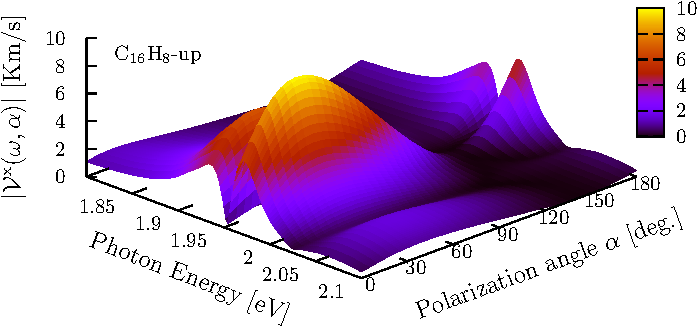
\includegraphics[width=\linewidth]{upplots/up-3d-vxb-2}}
    \\
    \subfigure[\ $|\mathcal{V}^{\mathrm{y}}|$ for \emph{up} structure 
    \label{fig:up-3d-vvy-2}]
    {
\includegraphics[width=\linewidth]{upplots/up-3d-vyb-2}}
    
    \caption{$|\mathcal{V}^{\mathrm{a}}(\omega,\alpha)|$ response vs. photon energy vs.
    polarization angle for the \emph{up} structure. The local maxima of both
    responses $|\mathcal{V}^{\mathrm{x}}(\omega,\alpha)|$ and
    $|\mathcal{V}^{\mathrm{y}}(\omega,\alpha)|$ are localized in the energy range from
    1.95\,eV to 2.00\,eV and for polarization angles from $25^{\circ}$ to
    $50^{\circ}$.}
    \label{fig:up-3d-vva-2}
\end{figure}
\begin{figure}[t]
    \centering
    \subfigure[\ $|\mathcal{V}^{\mathrm{x}}|$ \label{fig:up-vx-comp-rtp-2}]
    {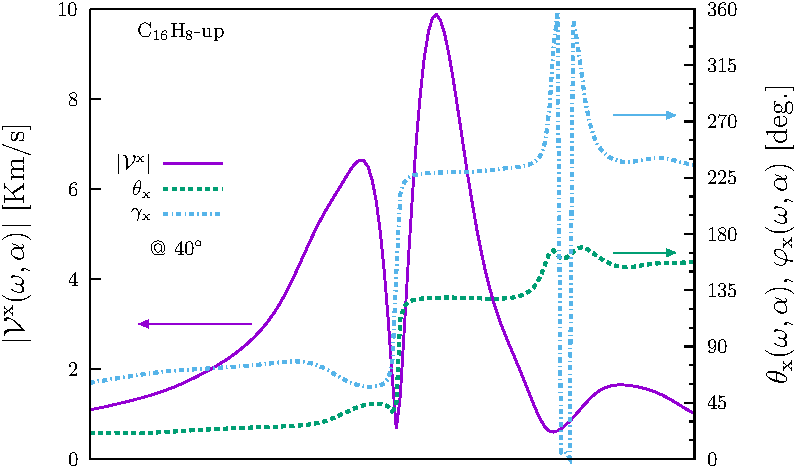
\includegraphics[width=\linewidth]{upplots/up-vxb-rtp-m2}}
    \\
    \subfigure[\ $|\mathcal{V}^{\mathrm{y}}|$ \label{fig:up-vy-comp-rtp-2}]
    {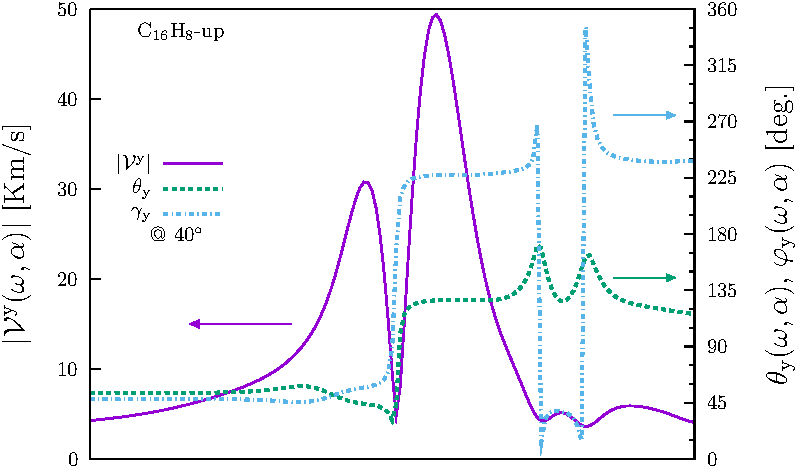
\includegraphics[width=\linewidth]{upplots/up-vyb-rtp-m2}}
    
    \caption{Intense response of
    $|\mathcal{V}^{\mathrm{x}}(\omega,\alpha)|$ and
    $|\mathcal{V}^{\mathrm{y}}(\omega,\alpha)|$ (top frames left scale of Figs. (a) and
    (b)), the corresponding polar $\varphi$ and azimuthal $\theta$ angles (top
    frames right scale), and the corresponding three components (bottom frames)
    for the \emph{up} structure fixing the polarization angle to
    $\alpha=40^{\circ}$ to maximize the response.}

    \label{fig:up-vab-comp-rtp-2}
\end{figure}
% %%%%%%%%%%%%%%%%%
% %% 1.8 eV - 2.0 eV
% %% Description of UP |V^{a}|, components and RTP
% %%%%%%%%%%%%%%%%%
From Fig. \ref{fig:up-vx-comp-rtp-1} we have that for an incoming bean with
energy of 0.088\,eV the three components have similar contributions and with
values of 
% 
$\mathcal{V}^{\mathrm{xx}}(\omega,\alpha)=-36.5$\,Km/s,
$\mathcal{V}^{\mathrm{xy}}(\omega,\alpha)=-23.2$\,Km/s, and
$\mathcal{V}^{\mathrm{xz}}(\omega,\alpha)= 39.8$\,Km/s 
% 
resulting in a value of
% 
$|\mathcal{V}^{\mathrm{x}}(\omega,\alpha)|=58.7$\,Km/s 
% 
being this value the absolute maximum obtained when the spin-velocity is fixed
in the $x$ direction. To this value corresponds a polar and azimuthal angles of
$\theta_{\mathrm{x}}(\omega,\alpha)=47$ and
$\varphi_{\mathrm{x}}(\omega,\alpha)=212$, respectively, being directed upper
the third Cartesian Quadrant of the $xy$ plane. Also from this figure we have
that those angle values are hold for almost all the peak of the response having
a deviation of $\pm 2^{\circ}$ in the range of energies from 0.028\,eV to
0.098\,eV from the corresponding to the absolute maximum mentioned before.
% 
Now, from Fig. \ref{fig:up-vy-comp-rtp-1} we have that the $\mathrm{yx}$ and
$\mathrm{yy}$ components have less contributions for the total response than the
$\mathrm{yz}$ and for the same incoming beam energy have values of
% 
$\mathcal{V}^{\mathrm{yx}}(\omega,\alpha)= -7.9$\,Km/s 
$\mathcal{V}^{\mathrm{yy}}(\omega,\alpha)=  8.6$\,Km/s, and
$\mathcal{V}^{\mathrm{yz}}(\omega,\alpha)= 87.2$\,Km/s 
% 
resulting in a value of the total response of
% 
$|\mathcal{V}^{\mathrm{y}}(\omega,\alpha)|=87.9$\,Km/s
% 
being this value the absolute maximum obtained when the spin-velocity is fixed
in the $y$ direction and being 1.5 times more intense than
$|\mathcal{V}^{\mathrm{x}}(\omega,\alpha)|$ To this absolute maximum correspond
spin polar and azimuthal angles $\theta_{\mathrm{y}}(\omega,\alpha)=8$ and
$\varphi_{\mathrm{y}}(\omega,\alpha)=133$, respectively, being directed almost
perpendicularly over the $xy$ plane and being localized on the first Cartesian
Quadrant. In a different way than in the
$|\mathcal{V}^{\mathrm{x}}(\omega,\alpha)|$ case only the polar angle is hold
for the peak of the response having a deviation of $\pm 2^{\circ}$ since the
onset to a energy value of 0.106\,eV but the azimuthal angle changes since the
onset to 0.106\,eV from $99^{\circ}$ to $176^{\circ}$.
% 
We also found that since the onset of the response till an energy for the
incoming beam of 0.118\,eV the components of both,
$|\mathcal{V}^{\mathrm{x}}(\omega,\alpha)|$ and
$|\mathcal{V}^{\mathrm{y}}(\omega,\alpha)|$ have no change in the spin
polarization direction. Finally, after this energy value both goes to zero.
% %%%%%%%%%%%%%%%%%
% %% 1.80 eV - 2.10 eV
% %% Description of UP |V^{a}| 3D
% %%%%%%%%%%%%%%%%%
Also there is another energy range of interest for an incoming energy beam from
1.80\,eV to 2.10\,eV, corresponding to the THz and visible radiation, presented
in Fig. \ref{fig:up-3d-vva-2} where two local maxima of
$|\mathcal{V}^{\mathrm{x}}(\omega,\alpha)|$ and
$|\mathcal{V}^{\mathrm{y}}(\omega,\alpha)|$ are obtained for the \emph{up}
structure.
% 
From this figure we have that for the zone between the energy ranges from
1.92\,eV to 1.94\,eV and from 1.96\,eV to 1.98\,eV and for polarization angles
from $30^{\circ}$ to $45^{\circ}$ those two local maxima zones are held.
% 
We found that the two local maxima are obtained for an energy of the incident
beam energies of 1.934\,eV and 1.972\,eV fixing again the polarization angle to
$40^{\circ}$. 
% %%%%%%%%%%%%%%%%
% %% Starting description of UP |V^{x}|, components and RTP
% %%%%%%%%%%%%%%%%
In the top frames of Figs. \ref{fig:up-vx-comp-rtp-2} and 
% 
\ref{fig:up-vy-comp-rtp-2} we present in solid lines the results of
$|\mathcal{V}^{\mathrm{x}}(\omega,\alpha)|$ and
$|\mathcal{V}^{\mathrm{y}}(\omega,\alpha)|$, related to the left scale, fixing
the polarization angle to $\alpha=40^{\circ}$ for which the response is
maximized for the \emph{up} structure. In the same figures and frames we present
in dashed lines the corresponding polar ($\theta_{\mathrm{x}}(\omega,\alpha)$
and $\theta_{\mathrm{y}}(\omega,\alpha)$) and azimuthal
($\varphi_{\mathrm{x}}(\omega,\alpha)$ and
$\varphi_{\mathrm{y}}(\omega,\alpha)$) angles related to the right scale. In the
bottom frames of same figures we present the decomposition of the responses in
the three corresponding components $\mathcal{V}^{\mathrm{xx}}(\omega,\alpha)$,
$\mathcal{V}^{\mathrm{xy}}(\omega,\alpha)$,
$\mathcal{V}^{\mathrm{xz}}(\omega,\alpha)$ and
$\mathcal{V}^{\mathrm{yx}}(\omega,\alpha)$,
$\mathcal{V}^{\mathrm{yy}}(\omega,\alpha)$,
$\mathcal{V}^{\mathrm{yz}}(\omega,\alpha)$.
% 
We found that for both cases, the components have similar contributions and for
an incoming energy beam of 1.934\,eV  we have the first local maximum resulting
in a value of $|\mathcal{V}^{\mathrm{x}}(\omega,\alpha)|= 6.6$\,Km/s along the
$x$ direction  with polar and azimuthal spin polarization angles
$\theta_{\mathrm{x}}(\omega,\alpha)= 42^{\circ}$ and
$\varphi_{\mathrm{x}}(\omega,\alpha)=59^{\circ}$ having fluctuations but being
directed over the first Cartesian Quadrant of the $xy$ plane.
% 
For the spin moving along the $y$ direction we have a value of
$|\mathcal{V}^{\mathrm{y}}(\omega,\alpha)|=28.7$\,Km/s with polar and azimuthal
angles $\theta_{\mathrm{y}}(\omega,\alpha)=45^{\circ}$ and
$\varphi_{\mathrm{y}}(\omega,\alpha)=56^{\circ}$ having variations of
$\pm5^{\circ}$ for energy variations of $\pm0.01$\,eV and being directed over
the fir Cartesian Quadrant of the $xy$ plane.
% 
Alike, for an incoming energy beam of 1.972\,eV we found the second and more
intense local maxima with all the components of both responses having similar
contributions and resulting in values of
$|\mathcal{V}^{\mathrm{x}}(\omega,\alpha)|=9.9$\,Km/s and spin polarization
angles $\theta_{\mathrm{x}}(\omega,\alpha)=129^{\circ}$ and
$\varphi_{\mathrm{x}}(\omega,\alpha)=229^{\circ}$ being almost constant in the
width of the peak having variations of $\pm1^{\circ}$ for variations in energy
of $\pm0.01$\,eV and being directed downward the third Cartesian Quadrant of the
$xy$ plane.
% 
For the spin moving in the $y$ direction we have a value of
$|\mathcal{V}^{\mathrm{y}}(\omega,\alpha)|=49.4$\,Km/s with spin polarization
angles $\theta_{\mathrm{y}}(\omega,\alpha)=127^{\circ}$ and
$\varphi_{\mathrm{y}}(\omega,\alpha)=227^{\circ}$ being almost constant with
variations of $\pm1^{\circ}$ for variations in energy of $\pm1$\,eV and being
directed downward the third Cartesian Quadrant of the $xy$ plane.
% 
Finally we have that for bot energies
$|\mathcal{V}^{\mathrm{y}}(\omega,\alpha)|$ is more intense than
$|\mathcal{V}^{\mathrm{x}}(\omega,\alpha)|$ being 4.4 times more intense for
1.932\,eV and 5.0 times more intense for 1.972\,eV. Also all the components of
the responses keep the spin polarization positive till an energy of the incoming
beam equal to 1.954\,eV when the spin polarization changes the direction and
after an energy for the incoming beam equal to 2.05\,eV both responses goes to
zero.

%%%%%%%%%%%%%%%%%%%%%%%%%%%%%%%%%%%%%%%%%%%%%%%%%%%%%%%%%%%%%%%%%%%%%%%%%%%%%%
%%%%%%%%%%%%%%%%%%%%%%%%%%% Res: fixin vel Alt  %%%%%%%%%%%%%%%%%%%%%%%%%%%%%%%

\textbf{Alt structure.}
\begin{figure}[tb]
    \centering
    \subfigure[\ $|\mathcal{V}^{\mathrm{x}}|$ for \emph{alt} structure 
    \label{fig:alt-3d-vvx}]
    {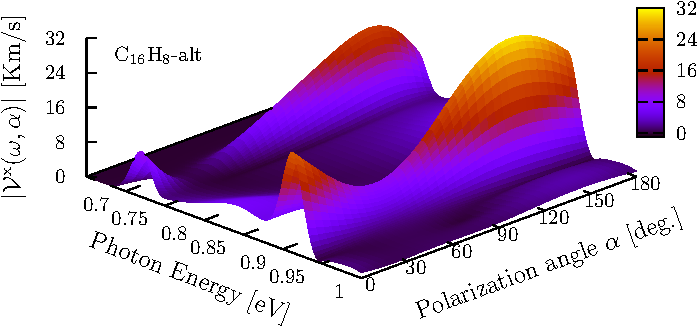
\includegraphics[width=\linewidth]{altplots/alt-3d-vxb}}
    \\
    \subfigure[\ $|\mathcal{V}^{\mathrm{y}}|$ for \emph{alt} structure 
    \label{fig:alt-3d-vvy}]
    {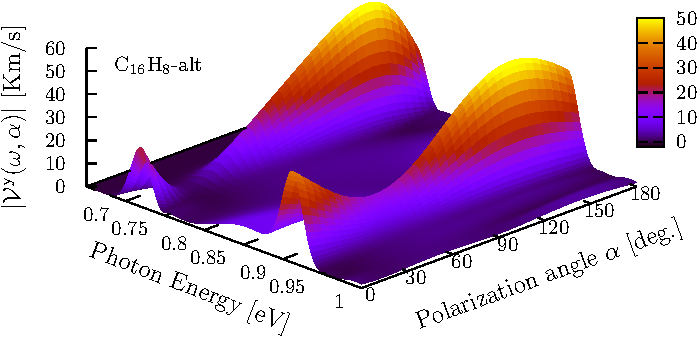
\includegraphics[width=\linewidth]{altplots/alt-3d-vyb}}
    
    \caption{$|\mathcal{V}^{\mathrm{a}}(\omega,\alpha)|$ response vs. photon
    energy vs. polarization angle for the \emph{alt} structure. The absolute
    maxima of both responses $|\mathcal{V}^{\mathrm{x}}(\omega,\alpha)|$ and
    $|\mathcal{V}^{\mathrm{y}}(\omega,\alpha)|$ are localized in the energy
    range from 0.90\,eV to 0.93\,eV and for polarization angles from
    120$^{\circ}$ to 150$^{\circ}$.}
    \label{fig:alt-3d-vva}
\end{figure}

\begin{figure}[tb]
    \centering
    \subfigure[\ $|\mathcal{V}^{\mathrm{x}}|$ \label{fig:alt-vx-comp-rtp}]
    {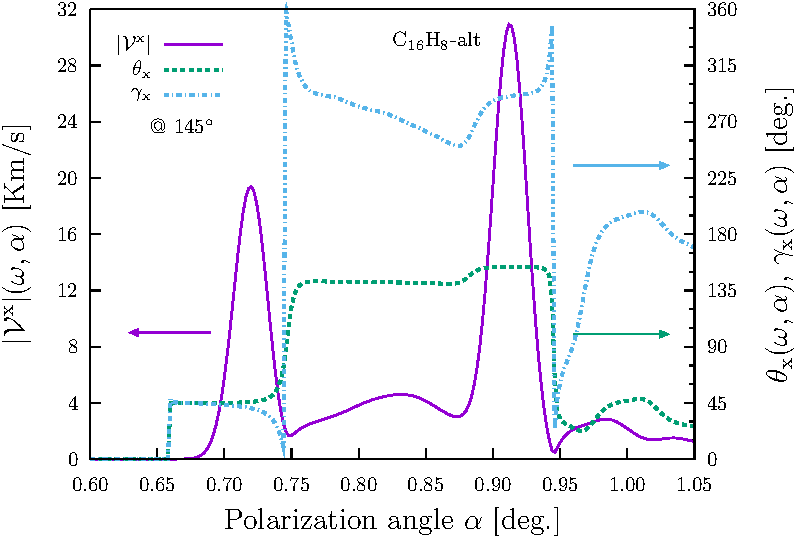
\includegraphics[width=\linewidth]{altplots/alt-vxb-rtp-m}}
    \\
    \subfigure[\ $|\mathcal{V}^{\mathrm{y}}|$ \label{fig:alt-vy-comp-rtp}]
    {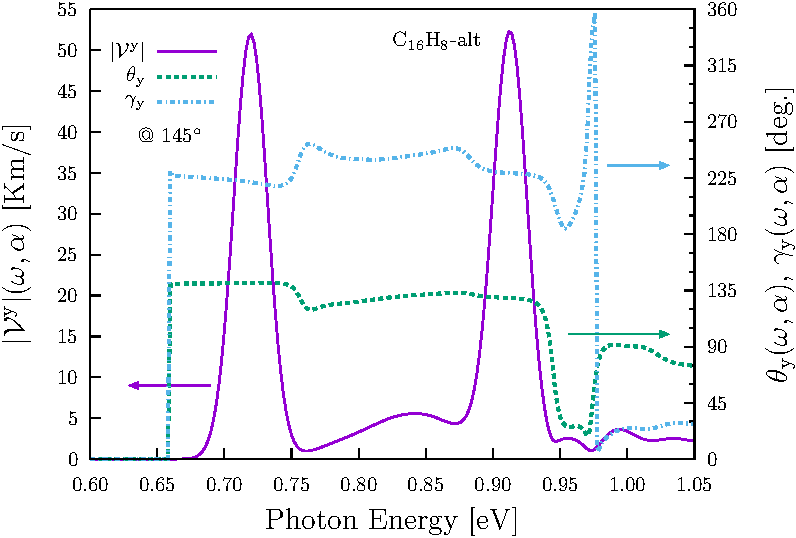
\includegraphics[width=\linewidth]{altplots/alt-vyb-rtp-m}}

    \caption{Most intense response of
    $|\mathcal{V}^{\mathrm{x}}(\omega,\alpha)|$ and
    $|\mathcal{V}^{\mathrm{y}}(\omega,\alpha)|$ (top frames left scale of Figs.
    (a) and (b)), the corresponding polar $\varphi$ and azimuthal $\theta$
    angles (top frames right scale), and the corresponding three components
    (bottom frames) for the \emph{alt} structure fixing the polarization angle
    to $\alpha=145^{\circ}$ to maximize the response.}
    \label{fig:alt-vab-comp-rtp}
\end{figure}

% %%%%%%%%%%%%%%%%%
% %% Description of ALT |V^{a}| 3D
% %%%%%%%%%%%%%%%%%
For the \emph{alt} structure we analyzed the energy range from 0.6\,eV to
1.0\,eV, corresponding to the THz radiation, where we found the a local maxima
and the most intense responses for $|\mathcal{V}^{\mathrm{x}}(\omega,\alpha)|$
and $|\mathcal{V}^{\mathrm{a}}(\omega,\alpha)|$. In Fig. \ref{fig:alt-3d-vva} we
present the $|\mathcal{V}^{\mathrm{a}}(\omega,\alpha)|$ spectra resulting from
evaluate again Eq. \eqref{eq:vv-mag} using different polarization angles
$\alpha$ in Eq. \eqref{eq:vab} but now for the \emph{alt} structure. We can see
that the onset of the response is when the energy of the incoming light is the
same of the gap energy.
%
From this picture we can see that for the zone between the energy range of
0.90\,eV-0.93\,eV and polarization angles between 120$^{\circ}$ and
150$^{\circ}$ is the zone where the maximum response for both,
$|\mathcal{V}^{\mathrm{x}}(\omega,\alpha)|$ and
$|\mathcal{V}^{\mathrm{y}}(\omega,\alpha)|$ is held. We also found that the
first peak is obtained when the energy of the incoming beam is 0.720\,eV and
the absolute maximum of the response is obtained when for 0.912\,eV, both for a
polarization angle $\alpha = 145^{\circ}$.
% %%%%%%%%%%%%%%%%
% %% Starting description of ALT |V^{a}|, components and RTP
% %%%%%%%%%%%%%%%%
In the top frames of Figs. \ref{fig:alt-vx-comp-rtp}  and 
%
\ref{fig:alt-vy-comp-rtp} we present in solid lines the results of
$|\mathcal{V}^{\mathrm{x}}(\omega,\alpha)|$ and
$|\mathcal{V}^{\mathrm{y}}(\omega,\alpha)|$, related to the left scale, fixing
the polarization angle to $\alpha=145^{\circ}$ for which the response is
maximized for the \emph{alt} structure. In the same figures and frames we
present ind dashed lines the spin polarization angles related to the right scale
and in the bottom frames the corresponding three components.
% 
Making the analysis for the components and angles when the spin current is
directed in the $x$ direction, corresponding to the Fig.
% 
\ref{fig:alt-vx-comp-rtp}, we found that for the \emph{alt} structure when the
energy of the incoming beam is 0.720\,eV we have similar contributions from all
the components resulting in a response of
$|\mathcal{V}^{\mathrm{x}}(\omega,\alpha)|=19.4$\,Km/s and polar and azimuthal
spin polarization angles $\theta_{\mathrm{x}}(\omega,\alpha)=46^{\circ}$ and
$\varphi_{\mathrm{x}}(\omega,\alpha)=41^{\circ}$ having variations in the range
of the peak but being directed over the first Cartesian Quadrant of the $xy$
plane;
% 
for an energy of 0.912\,eV we have a major contribution from the
$\mathcal{V}^{\mathrm{xz}}(\omega,\alpha)$ component resulting in a total
response of $|\mathcal{V}^{\mathrm{x}}(\omega,\alpha)|=30.9$\,Km/s and angles
$\theta_{\mathrm{x}}(\omega,\alpha)=154^{\circ}$, and
$\varphi_{\mathrm{x}}(\omega,\alpha)=290^{\circ}$ having variations of
$\pm3^{\circ}$ in for energy variations of $\pm1$\,eV and being directed
downward the fourth Cartesian Quadrant of the $xy$ plane.
% 
Making now the analysis for the components and angles when the spin current is
directed along the $y$ direction, corresponding to the Fig.
% 
\ref{fig:alt-vy-comp-rtp}, we found that when the energy of the incoming beam is
0.720\,eV we have more contribution from the
$\mathcal{V}^{\mathrm{yz}}(\omega,\alpha)$ component resulting in a response of
$|\mathcal{V}^{\mathrm{y}}(\omega,\alpha)|=51.9$\,Km/s and angles
$\theta_{\mathrm{y}}(\omega,\alpha)=141^{\circ}$ and
$\varphi_{\mathrm{y}}(\omega,\alpha)=222^{\circ}$ being the first constant and
the second having variations of $\pm3^{\circ}$ for energy variations of
$\pm0.3$\,eV and being directed downward the third Cartesian Quadrant of the
$xy$ plane.
% 
Then, for the peak centered at 0.912\,eV we have similar contributions of all
the components resulting in a response
$|\mathcal{V}^{\mathrm{y}}(\omega,\alpha)|=52.3$\,Km/s being this the absolute
maximum response for the \emph{alt} structure. The corresponding angles are
$\theta_{\mathrm{y}}(\omega,\alpha)=129^{\circ}$ and
$\varphi_{\mathrm{y}}(\omega,\alpha)=229^{\circ}$ being both constant for the
energy range of the peak and being directed downward the third Cartesian
Quadrant of the $xy$ plane.
% 
Finally we have that the three components of $|\mathcal{V}^{\mathrm{y}}|$ are
negative keeping the same spin polarization since the onset of the response to a
energy of the incoming beam of 0.886\,eV when the response decreases and goes to
zero.

%%%%%%%%%%%%%%%%%%%%%%%%%%%%%%%%%%%%%%%%%%%%%%%%%%%%%%%%%%%%%%%%%%%%%%%%%%%%%%
%%%%%%%%%%%%%%%%%%%%%%%%%% Res: Layer-by-layer  %%%%%%%%%%%%%%%%%%%%%%%%%%%%%%
%%%%%%%%%%%%%%%%%%%%%%%%%%%%%%%%%%%%%%%%%%%%%%%%%%%%%%%%%%%%%%%%%%%%%%%%%%%%%%

\section{Layer-by-layer analysis} % (fold)
\label{sec:res-layer_by_layer_analysis}

The structures presented here where divided into layers to analyze the he
layer-by-layer contribution for $\mathcal{V}^{\mathrm{ab}}$ response. The
\emph{alt} structure was divided in six layers corresponding the first one to
the top hydrogen atoms, from the second to the forth to carbon atoms in
different $z$ positions, and the sixth and last one to the bottom hydrogen
atoms. The \emph{up} structure was divided into two layers, the first one
comprised by the top hydrogen atoms and the second by the carbon atoms. The
layer divisions and atom positions for the unit cells are shown in Tables
\ref{tab:alt-unitcell} and \ref{tab:up-unitcell}.

% %%%%%%%%%%%%%%%%
% %% Description of Up layer |V^{yz}|
% %%%%%%%%%%%%%%%%
\begin{figure}[t]
    \centering
    \subfigure[\ \label{fig:up-vyz-lay-1}]
    {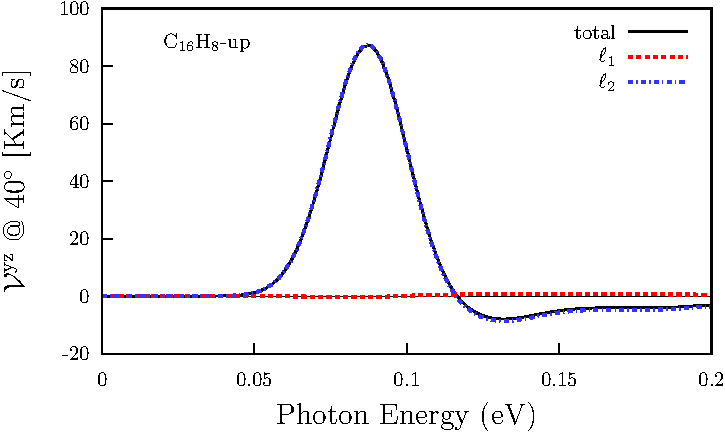
\includegraphics[width=\linewidth]{upplots/up-vyz-layers-1}}
    \\
    \subfigure[\ \label{fig:up-vyz-lay-2}]
    {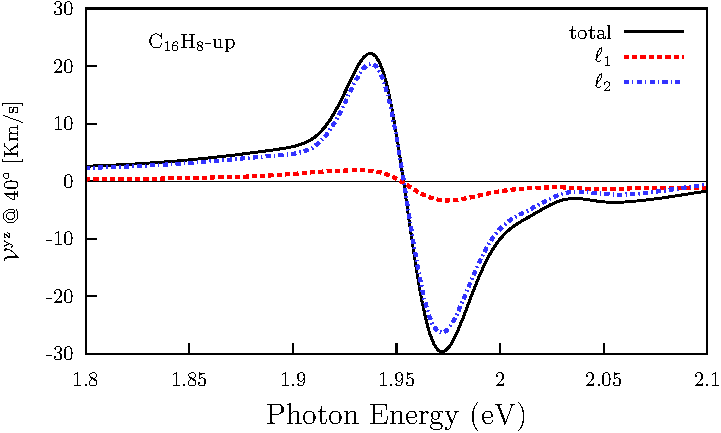
\includegraphics[width=\linewidth]{upplots/up-vyz-layers-2}}
    
    \caption{Layer-by-layer contribution of $\mathcal{V}^{\mathrm{yz}}$ for the
     \emph{up} structure.}
    \label{fig:up-vyz-lay}
\end{figure}

From the bottom frames of Figs. \ref{fig:up-vab-comp-rtp-1} and 
% 
\ref{fig:up-vab-comp-rtp-2} we can see that for the \emph{up} structure again
the most intense component of $|\mathcal{V}^{\mathrm{x}}|$ and
$|\mathcal{V}^{\mathrm{y}}|$ corresponds to $\mathcal{V}^{\mathrm{yz}}$ which
has a value of 87.2\,Km/s for an energy incident beam of 0.088\,eV and
-29.7\,Km/s for an energy incident beam of 1.972\,eV. This component and the
corresponding layer by layer contribution is depicted in Fig. 
\ref{fig:up-vyz-lay}s.
% 
From this figure we have that for the energy range from 0\,eV to 0.2\,eV the
response comes from the second layer composed by carbon atoms presented in Tab.
\ref{tab:up-unitcell} and denoted by the number 2 in Fig. \ref{fig:up-struc}. In
the other hand, the response for the energy range from 1.8\,eV to 2.1\,eV almost
all the response comes from the carbon atoms having a leaser contribution from
the hydrogen layer.
% %%%%%%%%%%%%%%%%
% %% Description of ALT layer |V^{yz}|
% %%%%%%%%%%%%%%%%
From the bottom frames of Fig. \ref{fig:alt-vab-comp-rtp} we can see that for
the \emph{alt} structure the most intense component of
$|\mathcal{V}^{\mathrm{x}}|$ and $|\mathcal{V}^{\mathrm{y}}|$ corresponds to
$\mathcal{V}^{\mathrm{yz}}$ which has a value of -40.2\,Km/s for an
energy incident beam of 0.72\,eV. This component and the corresponding layer by
layer contribution is depicted in Fig. \ref{fig:alt-vyz-lay}. From this figure
we have that for the energy range from 0.70\,eV to 0.74\,eV the fifth and sixth
layers corresponding to the bottom carbon and hydrogen numbered with 5 and 6 in
Fig. \ref{fig:alt-struc} have contributions in opposite direction than the other
4 layers resulting in a total response $\mathcal{V}^{\mathrm{yz}}= -40.2$\,Km/s
for an incoming beam energy of 0.72\,eV. In the other hand, for the energy range
from 0.88\,eV to 0.95\,eV the response for the all six layers the responses are
in the same direction resulting in a total response
$\mathcal{V}^{\mathrm{yz}}=-32.89$\,Km/s for an incoming beam with energy of
0.912\,eV.
\begin{figure}[b]
    \centering
    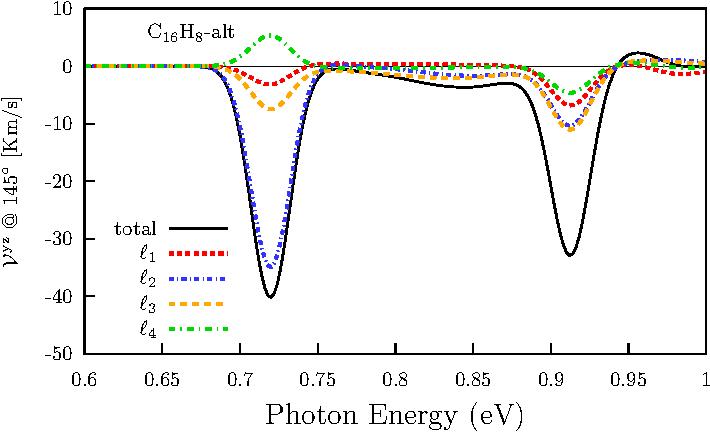
\includegraphics[width=\linewidth]{altplots/alt-vyz-layers}
    
    \caption{Layer-by-layer contribution of $\mathcal{V}^{\mathrm{yz}}$ for the
     \emph{alt} structure.}
    \label{fig:alt-vyz-lay}
\end{figure}


\bibliography{article.bib}

\end{document}

















